\section{Three Measurement Illusions}
\label{sec:illusions}

\subsection{Leniency hides discrimination}
\label{sec:lenient}

A binary verdict with hit rate $H$ (the share of wrong attempts it flags) and false-alarm rate $F$ has
\begin{equation}
\mathrm{AUROC}=\tfrac12\,(1+H-F),
\end{equation}
which is close to $\tfrac12$ whenever the judge rarely says ``incorrect'', whatever its discrimination. In Phase~2
the mixed judge flagged $7.4\%$ of wrong own attempts and $2.2\%$ of right ones. That gives an AUROC of $0.526$ (reported
as $0.53$, ``near chance''). In signal-detection terms it is $d'=z(H)-z(F)=0.57$.

Fitting Eq.~\ref{eq:judge} to these two rates gives $c_0=2.05$ and $d=0.80$. With no further fitting the same judge
predicts AUROC $0.568$ with four sampled verdicts, the value later measured for that judge on test attempts. Its
latent score has AUROC $0.715$.

Moving only $c_0$, to about $28\%$ ``incorrect'' verdicts, raises the four-verdict AUROC to $0.665$, the value
reached by self-judge training on a $49\%$-wrong training set. The training ``gain'' is therefore reproduced by a
criterion shift, with discrimination unchanged. Section~\ref{sec:stage0} tests this account directly.

\subsection{Pooled AUROC is between-question AUROC}
\label{sec:pooled}

Split the pairs behind a pooled AUROC into same-question and cross-question pairs. With $k_x$ right attempts out of
$N$ on question $x$, and $K=\sum_x k_x$ over $Q$ questions,
\begin{equation}
\begin{gathered}
A_{\text{pooled}} = w A_{\text{within}} + (1-w) A_{\text{between}},\\
w=\frac{\sum_x k_x(N-k_x)}{K(QN-K)}.
\end{gathered}
\end{equation}
In expectation
$w\approx\frac{N-1}{NQ}\cdot\frac{\mathbb E[p(1-p)]}{\bar p(1-\bar p)}$, which falls like $1/Q$. On a $400\times4$
pool, $w=0.076\%$, so the pooled AUROC is a between-question AUROC. A score that knows only $p_x$, and nothing about
the attempt, reaches pooled AUROC $0.94$. \citet{bulut2026problem} report the same confound for hidden-state probes.

The next result says why this matters.

\paragraph{Theorem 1 (invariance).}
Let $f_i\in[0,1]$ flag attempt $i$ for resampling. The expected change in accuracy is
\begin{equation}
\Delta=\mathbb E[f\,(p_x-Z)]=-\mathbb E_x\big[\mathrm{Cov}(f,Z\mid x)\big].
\end{equation}
For selection, the Bayes-optimal choice among a question's answers depends on the verifier only through the
within-question likelihood ratios $\Lambda_x(s)=f(s\mid x,Z{=}1)/f(s\mid x,Z{=}0)$.

\emph{Proof.} Appendix~\ref{app:proofs}.

\emph{Consequences.}
\begin{itemize}
\item Any flag or score that depends only on the question has $\Delta=0$ exactly and reduces selection to majority
  vote, whatever its pooled AUROC.
\item Random flags have $\Delta=0$ (Phase~2: $69.75\to69.75$).
\item The optimal flag is question-relative: flag iff $P(Z{=}1\mid x,s)<p_x$.
\end{itemize}
Figure~\ref{fig:auroc} shows the point in the model. Raising the difficulty signal moves pooled AUROC from $0.50$ to
$0.75$ with no gain in picking, while picking accuracy is a single curve in the within-question AUROC.

\begin{figure}[t]
\centering
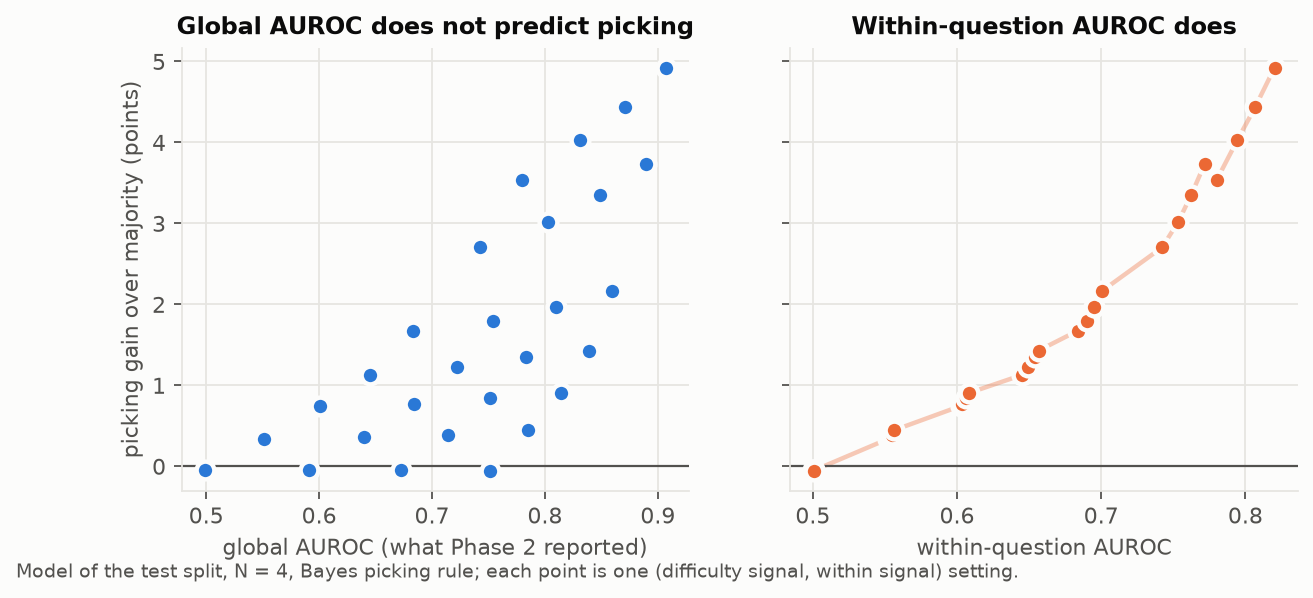
\includegraphics[width=\columnwidth]{figures/fig1_auroc_vs_gain.png}
\caption{Picking gain over majority vote in the calibrated model ($N=4$, Bayes rule). Left: against pooled AUROC.
Right: against within-question AUROC.}
\label{fig:auroc}
\end{figure}

\subsection{Most of the headroom is ties}
\label{sec:headroom}

At $N=4$ the 8.7-point gap between majority vote and pass@4 splits as follows:
\begin{itemize}
\item \textbf{Ties (5.7 points):} configurations such as (right, wrong, wrong, wrong) all different, where majority
  vote is a coin flip.
\item \textbf{Overturns (3.0 points):} the right answer has to beat a larger wrong group.
\end{itemize}

\paragraph{Proposition 1 (tie-breaking).}
Take majority vote and let the judge decide only among tied groups. If right scores are $\mathcal N(d,1)$ and wrong
scores $\mathcal N(0,1)$, independently, then
\begin{equation}
\begin{split}
\mathrm{gain}={}&P_{1\text{-}1\text{-}1\text{-}1}\Big(M_4(d)-\tfrac14\Big)\\
&+P_{2\text{-}2}\Big(\Phi(d)-\tfrac12\Big)\ \ge 0,
\end{split}
\end{equation}
where $M_4(d)=\int\phi(t-d)\Phi(t)^3\,dt$ and $P_{\cdot}$ are the configuration shares ($6.7\%$ and $1.3\%$ on
test). The closed form matches simulation to within $0.07$ points.

By contrast, Phase~2's summed-confidence rule can fall below majority vote: a single confident wrong attempt can
outscore two right ones.

Overturning a plurality of $m$ with a single right attempt under the Bayes rule (vote weight $\beta$) succeeds with
probability $\Phi\big([(1-m)\beta+(1+m)d^2/2]/(\sqrt{1+m}\,d)\big)$, which is small for weak judges.

The headroom also sits on hard questions: mean solve rate $0.33$, against $0.54$ for the pairs a within-question AUROC
averages over. We therefore report within-question AUROC on \emph{contested} questions, where majority vote does not
already pick the right answer.
